\section{Probabilidade e Estatística}

\questao{(OM$^3$SP 2026 - 1$^\circ$ fase) O professor de Educação Física, Henry, vai realizar um jogo e para formar dois times de 10 jogadores cada ele tem para sorteio 10 fichas verdes numeradas de 1 a 10 e 10 fichas amarelas também numeradas de 1 a 10. Qual é a probabilidade de um estudante retirar uma ficha com o número 8?}

        \begin{multicols}{4}
            \begin{enumerate}[label=\alph*)]
                \item $\dfrac{2}{10}$
                \item $\dfrac{1}{20}$
                \item $\dfrac{2}{8}$
                \item $\dfrac{1}{10}$
            \end{enumerate}
        \end{multicols}

\begin{solucoes}{1}
    \solucao
    Observando a situação, temos um total de 20 fichas, 10 de cada cor, signfica que cada número irá aparecer duas vezes, incluindo o número 8, desta forma, temos que a probabilidade de algum estudante escolher o número 8 é duas de um total de 20, temos:

$\begin{WithArrows}[tikz={>=stealth, text width = 6cm, draw=black!70, text=black!70}, interline=2mm]
    P =& \dfrac{2}{20} \Arrow[ll]{Simplificando, temos a seguinte fração}\\
    P =& \dfrac{1}{10}
\end{WithArrows}$

Então, a probabilidade de algum estudante retirar o número 8 é de $\dfrac{1}{10}$.

\textbf{ALTERNATIVA D}


\end{solucoes}

\questao{ O professor de Matemática Tony da Escola Marcelo Minervo dos Santos Pimentel organizou em um gráfico os dados referentes à última avaliação dos estudantes do 9$^\circ$ ano A, analise a seguir.}

        \begin{center}
            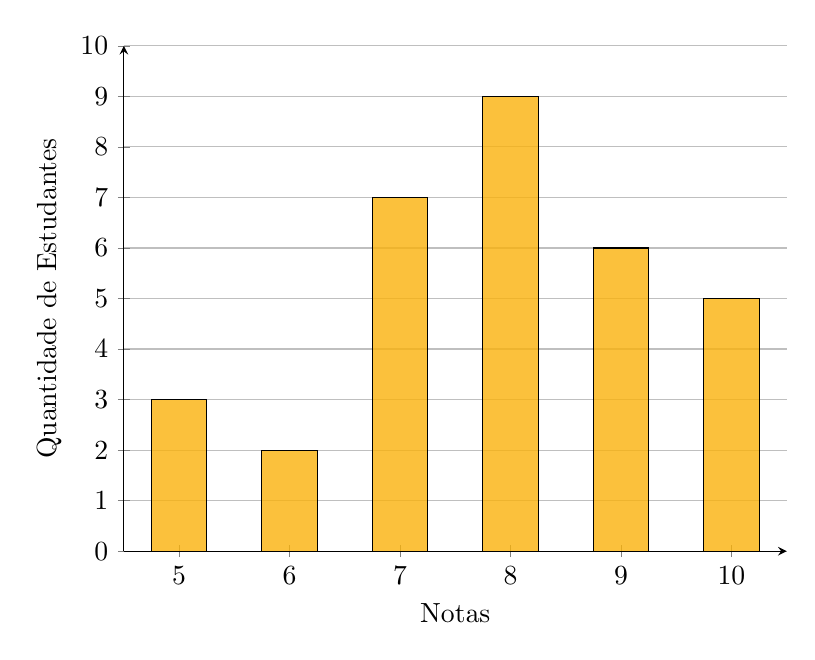
\begin{tikzpicture}
                \begin{axis}[
                        ybar,
                        ytick distance=1,
                        ymax=10,
                        bar width=10pt,
                        xlabel={Notas},
                        ylabel={Quantidade de Estudantes},
                        symbolic x coords={5,6,7,8,9,10},
                        xtick=data,
                        ymin=0,
                        grid=major,
                        xmajorgrids=false,
                        axis lines=left,
                        bar width=20pt,
                        enlarge x limits=0.1,
                        width=10cm,
                        height=8cm,
                    ]
                    \addplot[
                        fill=yellow!40!orange,
                        fill opacity=.8
                    ] coordinates{
                        (5,3) (6,2) (7,7) (8,9) (9,6) (10,5)
                    };
                \end{axis}
            \end{tikzpicture}
        \end{center}

        Quantos estudantes participaram dessa avaliação?

        \begin{multicols}{2}
            \begin{enumerate}[label=\alph*)]
                \item 30 Estudantes
                \item 35 Estudantes
                \item 32 Estudantes
                \item 33 Estudantes
            \end{enumerate}
        \end{multicols}

\begin{solucoes}{1}
    \solucao

    De acordo com o gráfico, temos o valor das notas no eixo horizontal e a quantidade de alunos no eixo vertical, então para saber a quantidade total de estudantes que participaram nessa avaliação, somamos a quantidade de estudantes em cada nota obtida, assim temos:

$\begin{WithArrows}[tikz={>=stealth, text width = 6cm, draw=black!70, text=black!70}, interline=2mm]
    nota\, 5 :&\, 3\, estudantes \\
    nota\, 6 :&\, 2\, estudantes \\
    nota\, 7 :&\, 7\, estudantes \\
    nota\, 8 :&\, 9\, estudantes \\
    nota\, 9 :&\, 6\, estudantes \\
    nota\, 10:&\, 5\, estudantes \\ \hline
              &\, 32\, estudantes
\end{WithArrows}$

Sendo assim, \textbf{32 estudantes} realizaram à ultima avaliação do professor Tony.

\textbf{ALTERNATIVA C}
\end{solucoes}
